\documentclass[11pt]{article}
%\usepackage{booktabs}
%\usepackage{caption}
\usepackage{float}

\usepackage{geometry}                		% See geometry.pdf to learn the layout options. There are lots.
\geometry{letterpaper}                   		% ... or a4paper or a5paper or ... 
%\geometry{landscape}                		% Activate for for rotated page geometry
%\usepackage[parfill]{parskip}    		% Activate to begin paragraphs with an empty line rather than an indent
\usepackage{graphicx}				% Use pdf, png, jpg, or eps§ with pdflatex; use eps in DVI mode
								% TeX will automatically convert eps --> pdf in pdflatex		
\usepackage{amssymb}

\title{Replication: Currie et al.: Fast-Food, Obesity, Weight Gain}
\date{}							% Activate to display a given date or no date

\begin{document}
\maketitle
%\section{}
%\subsection{}
\newpage
\begin{table}[H]
\caption{\label{fig: sum_stats} Summary Statistics for California School Data}
\vspace{-0.3cm}

\begin{center}\tiny
{
\def\sym#1{\ifmmode^{#1}\else\(^{#1}\)\fi}
\begin{tabular}{l*{4}{c}}
\hline\hline
                    &\multicolumn{1}{c}{All}&\multicolumn{1}{c}{$<$0.5 miles FF}&\multicolumn{1}{c}{$<$0.25 miles FF}&\multicolumn{1}{c}{$<$0.1 miles FF }\\
\hline
Number of obese students&     366.275&     384.300&     383.048&     400.746\\
\\ \textit{School Characteristics}&            &            &            &            \\
School qualified for title 1 funding&       0.397&       0.411&       0.406&       0.436\\
Number of students  &    1566.184&    1663.978&    1663.624&    1715.707\\
Student teacher ratio&      22.393&      22.841&      22.668&      22.857\\
Share black students&       0.084&       0.093&       0.093&       0.086\\
Share asian students&       0.107&       0.117&       0.118&       0.116\\
Share hispanic students&       0.380&       0.409&       0.416&       0.436\\
Share native american students&       0.014&       0.010&       0.010&       0.012\\
Share immigrant students&       0.034&       0.029&       0.030&       0.033\\
Share female students&       0.475&       0.477&       0.477&       0.490\\
Share eligible for free lunch&       0.290&       0.306&       0.313&       0.311\\
Share eligible for subsidised lunch&       0.063&       0.064&       0.063&       0.063\\
FTE teachers per student&       0.048&       0.047&       0.047&       0.047\\
Average test scores for 9th grade&      56.255&      54.964&      54.737&      52.291\\
Test score information missing&       0.024&       0.020&       0.022&       0.016\\
 \\  \textit{School District Characteristics}&            &            &            &            \\
Students teacher ratio&      20.897&      21.095&      20.911&      21.092\\
Share immigrant students&       0.028&       0.025&       0.025&       0.028\\
Share non-English speaking students&       0.206&       0.224&       0.225&       0.222\\
Share IEP students  &       0.126&       0.125&       0.132&       0.120\\
Staff student ratio &       0.102&       0.099&       0.102&       0.095\\
Share diploma recipients&       0.086&       0.084&       0.082&       0.091\\
Share diploma recipients missing&       0.004&       0.004&       0.008&       0.000\\
\\  \textit{Census Demographics} &            &            &            &            \\
Median household income in 1999&   48596.074&   45686.657&   44183.090&   44691.683\\
Median earnings in 1999 for popn >=16 with earnings&   25674.202&   24668.101&   24271.405&   23942.224\\
Average household size for all occupied housing units&       2.967&       2.932&       2.840&       2.881\\
Median contract rent (dollars) for specified renter occupied housing&     743.736&     741.186&     734.136&     706.286\\
Median gross rent (dollars) for specified renter occupied housing&     835.741&     825.461&     812.538&     781.927\\
Median Value for all Owner Occupied Housing Units&  202783.236&  199823.654&  199834.384&  195244.011\\
Percent of the population that is white&       0.629&       0.597&       0.591&       0.578\\
Percent of the population that is white&       0.056&       0.062&       0.064&       0.053\\
Percent of the population that is asian&       0.090&       0.099&       0.098&       0.110\\
Percent of the population that is male&       0.491&       0.489&       0.487&       0.494\\
Percent of the population 15+ never married&       0.289&       0.310&       0.320&       0.314\\
Percent of the population 15+ married (spouse present or absent)&       0.546&       0.519&       0.505&       0.513\\
Percent of the population divorced&       0.103&       0.107&       0.111&       0.107\\
Percent of popn 25+ with just a high school diploma&       0.220&       0.219&       0.219&       0.220\\
Percent of popn 25+ with some college, no degree&       0.235&       0.226&       0.223&       0.219\\
Percent of popn 25+ with Associate's degree&       0.072&       0.069&       0.071&       0.072\\
Percent of popn 25+ with Bachelor's degree&       0.150&       0.149&       0.151&       0.139\\
Percent of popn 25+ with Graduate degree&       0.078&       0.076&       0.077&       0.069\\
Percent of popn 16+ in labor force&       0.616&       0.618&       0.619&       0.617\\
Percent of popn 16+ in labor force that is unemployed&       0.083&       0.085&       0.088&       0.079\\
Percent of households with income under 10k&       0.092&       0.099&       0.106&       0.101\\
Percent of households with income over 200k&       0.026&       0.022&       0.020&       0.020\\
Percent of households with wage or salary income&       0.782&       0.784&       0.784&       0.789\\
Percent of housing units occupied&       0.946&       0.953&       0.953&       0.950\\
Percent of population in owner-occupied units&       0.592&       0.530&       0.481&       0.488\\
Percent of housing units considered urban&       0.912&       0.974&       0.971&       0.987\\
\\  \textit{Outcome Variable} &            &            &            &            \\
Percent obese students&      32.949&      33.772&      33.724&      35.733\\
\hline\hline
\end{tabular}
}


\end{center}
\vspace{-0.3cm}
\par
\begin{minipage}{ \linewidth}
\scriptsize{Notes: This table lists all the controls used for the school regressions, with the exception of year and school fixed
effects.}
\end{minipage}

\end{table}



\begin{table}[H]
\caption{\label{fig: sum_stats} Summary Statistics for California School Data}
\vspace{-0.3cm}

\begin{center}\small
{
\def\sym#1{\ifmmode^{#1}\else\(^{#1}\)\fi}
\begin{tabular}{l*{4}{c}}
\hline\hline
                    &\multicolumn{4}{c}{Percent of ninth graders that are obese }                           \\
                    &\multicolumn{1}{c}{(1)}         &\multicolumn{1}{c}{(2)}         &\multicolumn{1}{c}{(3)}         &\multicolumn{1}{c}{(4)}         \\
\hline
Fast food within 0.10 miles&       3.081\sym{*}  &       1.737\sym{**} &       6.270\sym{**} &       6.334\sym{**} \\
                    &     (1.607)         &     (0.880)         &     (2.918)         &     (2.875)         \\
[1em]
Other restaurant within 0.10 miles&       0.682         &      -0.631         &       1.026         &       1.003         \\
                    &     (1.031)         &     (0.577)         &     (1.820)         &     (1.824)         \\
[1em]
Fast food within 0.25 miles&      -2.486\sym{**} &      -0.907\sym{*}  &      -1.830         &      -1.795         \\
                    &     (1.111)         &     (0.548)         &     (1.197)         &     (1.210)         \\
[1em]
Other restaurant within 0.25 miles&       2.142\sym{**} &       0.041         &       0.262         &       0.037         \\
                    &     (0.876)         &     (0.493)         &     (0.972)         &     (0.943)         \\
[1em]
Fast food within 0.5 miles&       1.390\sym{*}  &      -0.045         &      -1.089         &      -0.831         \\
                    &     (0.822)         &     (0.451)         &     (1.109)         &     (1.087)         \\
[1em]
Other restaurant within 0.5 miles&       1.227         &       0.539         &      -0.397         &      -0.415         \\
                    &     (0.841)         &     (0.493)         &     (0.871)         &     (0.816)         \\
\hline
Implied cumulative effect \\ to fast food restaurant within 0.1 miles&      1.9852         &       .7854         &      3.3519         &      3.7079         \\
 (standard errors)  &       1.509         &         .86         &       3.037         &       2.984         \\
School FE           &                     &                     &  \checkmark         &  \checkmark         \\
Year FE             &                     &  \checkmark         &                     &  \checkmark         \\
Census Controls     &                     &  \checkmark         &                     &  \checkmark         \\
School Controls     &                     &  \checkmark         &                     &  \checkmark         \\
N                   &        8373         &        8373         &        8373         &        8373         \\
R2                  &       0.021         &       0.417         &       0.644         &       0.651         \\
\hline\hline
\end{tabular}
}


\end{center}
\vspace{-0.3cm}
\par
\begin{minipage}{ \linewidth}
\scriptsize{Notes: This table lists all the controls used for the school regressions, with the exception of year and school fixed
effects.}
\end{minipage}

\end{table}



\begin{figure}[H]
\vspace{0.5cm}
\begin{center}
\caption{\label{fig: obes_schools} Impact of Fast Food on Obesity in Schools}
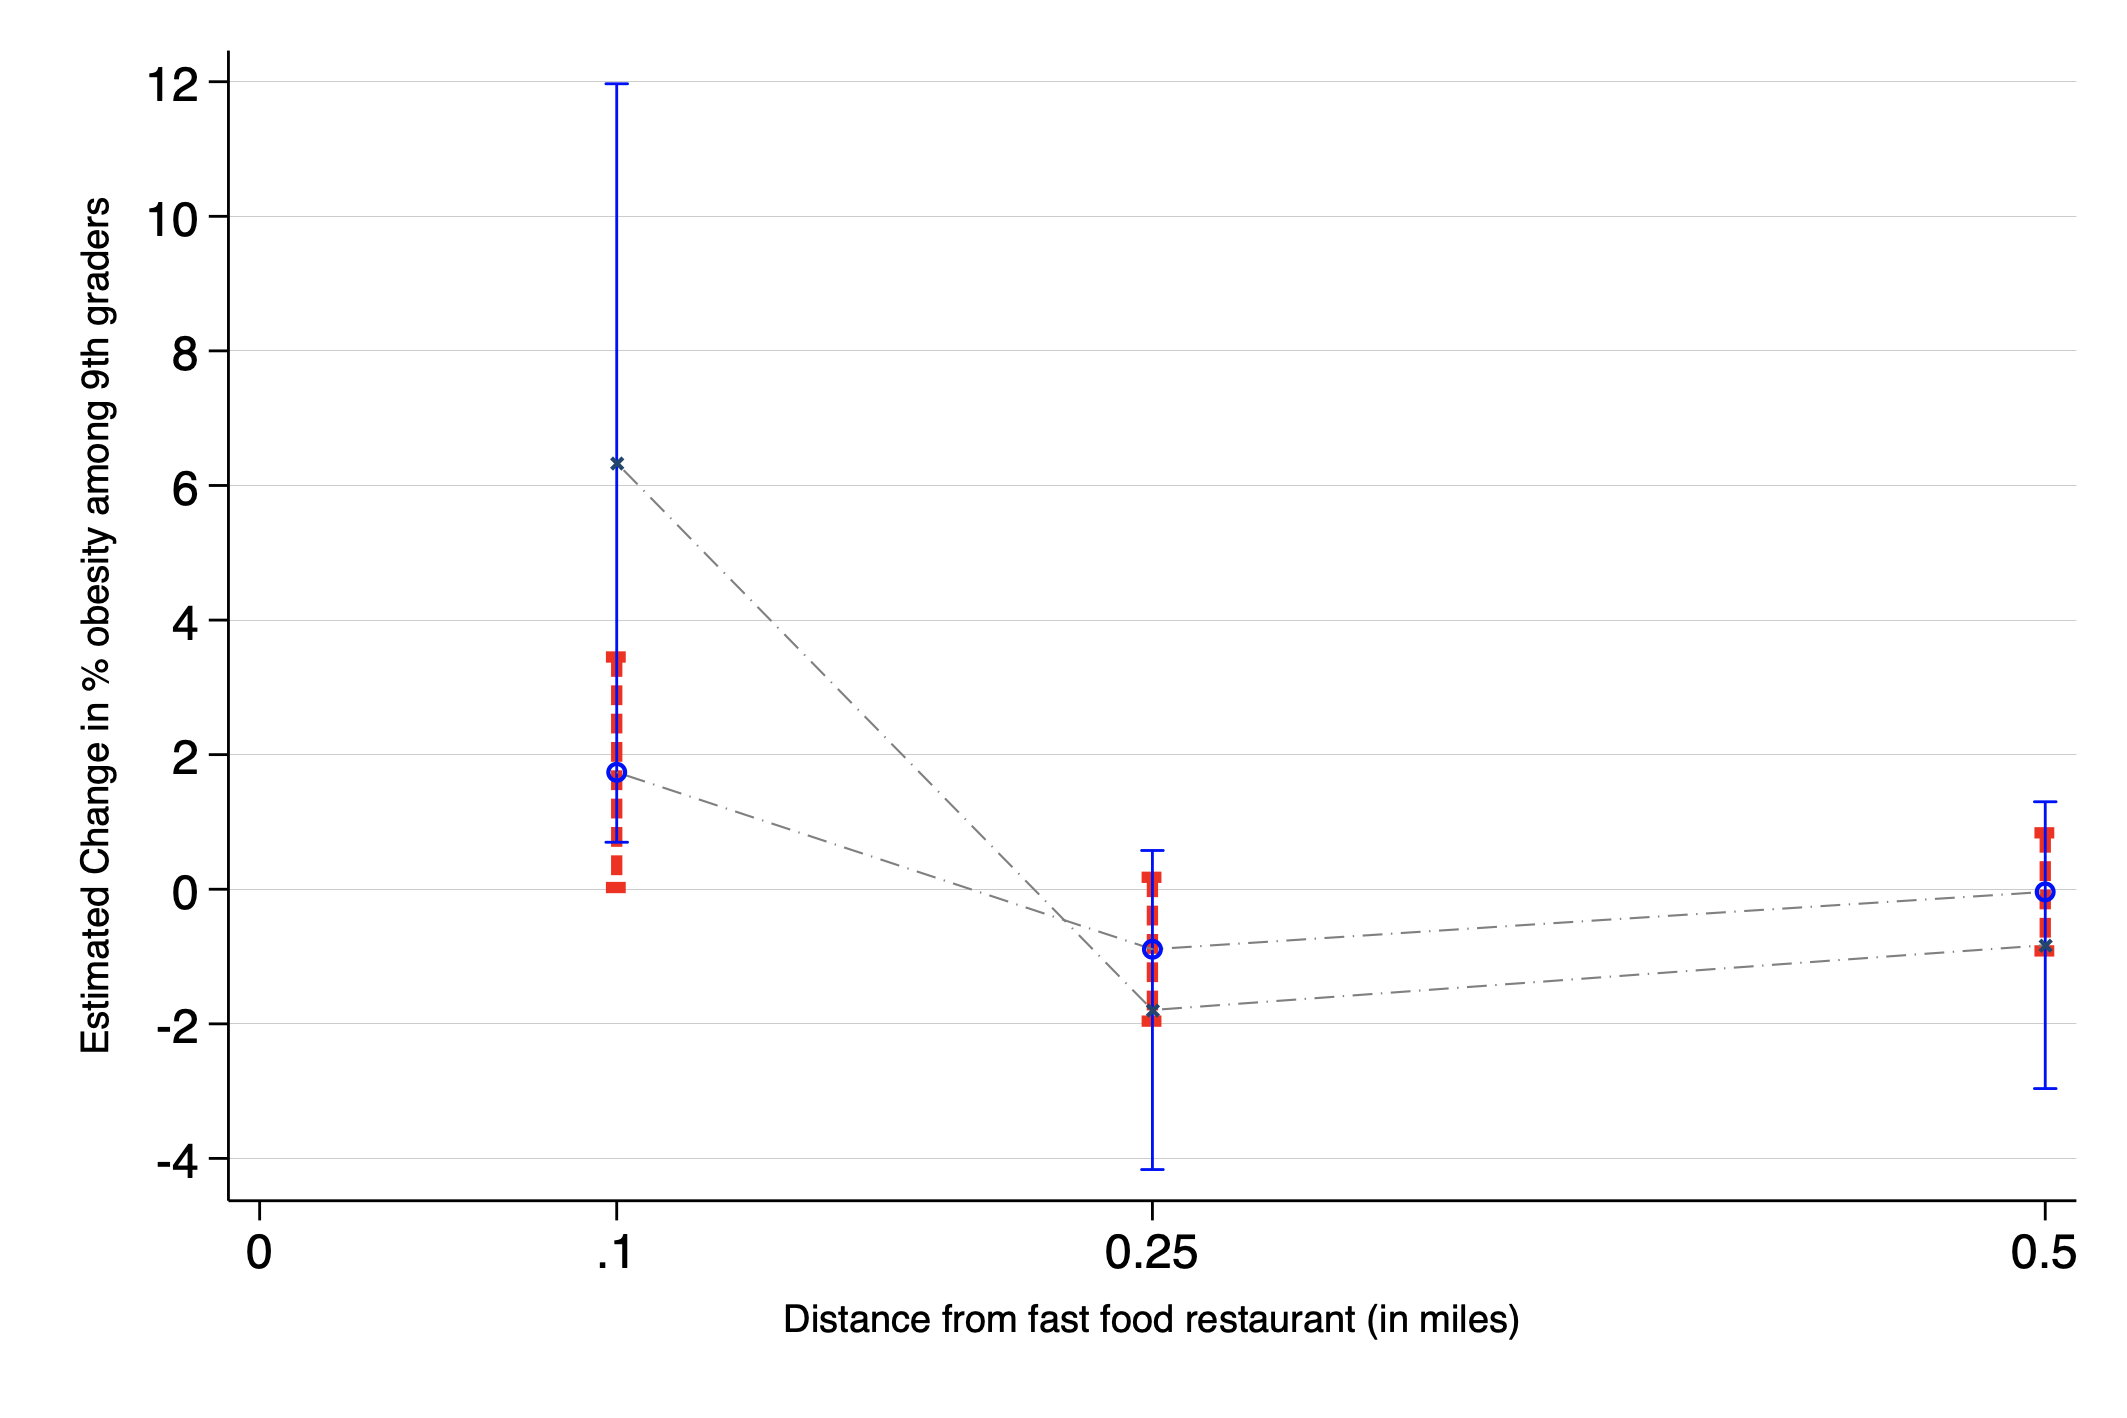
\includegraphics[width=130 mm, height=90 mm]{../figures/figure1A.png} 
\end{center}
\vspace{-0.3cm}
\par
\begin{minipage}{ \linewidth}
\scriptsize{Note: The blue vertical bar represent the 95 \% confidence interval using panel estimates; the red dashed vertical bar represent the 95 \% confidence interval using cross-sectional estimates}
\end{minipage}

\end{figure}




\end{document}  